\begin{figure}[t]
    \centering
    \begin{subfigure}[b]{0.8\linewidth}
        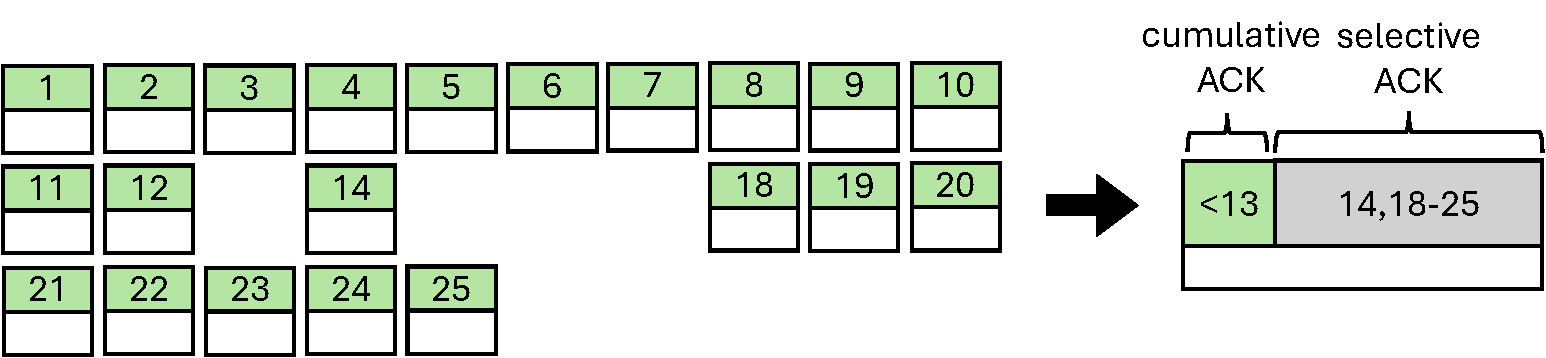
\includegraphics[width=\linewidth]{slides/figures/ack_cleartext.pdf}
        \caption{TCP packets with cleartext sequence numbers.}
        \label{fig:slides:ack-example:cleartext}
    \end{subfigure}
    \begin{subfigure}[b]{0.8\linewidth}
        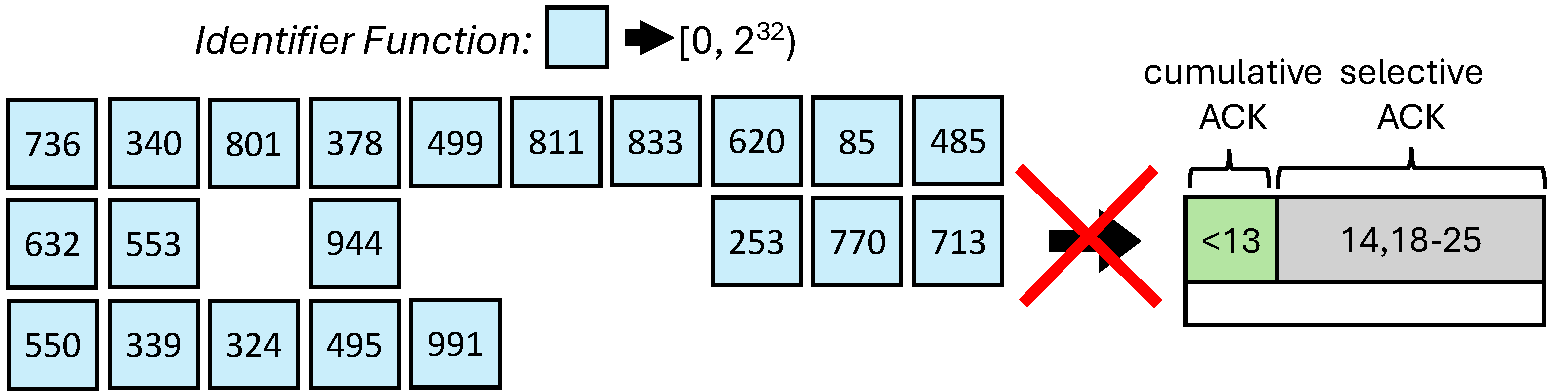
\includegraphics[width=\linewidth]{slides/figures/ack_encrypted.pdf}
        \caption{Randomly encrypted QUIC packets.}
        \label{fig:slides:ack-example:encrypted}
    \end{subfigure}
    \caption{Referring to a set of packets is easy when labeled with cleartext
    sequence numbers by using a cumulative and selective ACK. It is hard when
    the packets are randomly encrypted because there is no such concept of a
    range of packets or even a missing packet. The identifier function
    (\Cref{sec:quack:problem:identifiers}) deterministically
    maps a packet payload to a random 32-bit identifier.}
    \label{fig:slides:ack-example}
\end{figure}
